\documentclass[a4paper,titlepage]{article}
\usepackage{ascmac}
\usepackage{amsmath,amssymb}
\usepackage{siunitx}
\sisetup{group-separator = {,}}
\usepackage[dvipdfmx]{graphicx}

\usepackage{listings}
\usepackage{color}

\lstset{
language={Ruby},
basicstyle={\small\ttfamily},
identifierstyle={\small},
commentstyle={\small\ttfamily \color[rgb]{0,0.5,0}},
keywordstyle={\small\ttfamily\bfseries \color[rgb]{1,0,0}},
ndkeywordstyle={\small},
stringstyle={\small\ttfamily \color[rgb]{0,0,1}},
frame={tb},
breaklines=true,
columns=[l]{fullflexible},
numbers=left,
xrightmargin=0zw,
xleftmargin=3zw,
numberstyle={\scriptsize},
stepnumber=1,
numbersep=1zw,
morecomment=[l]{//}
}

\newcommand{\Cost}{\mathrm{Cost}}
\newcommand{\Price}{\mathrm{Price}}
\newcommand{\Power}{\mathrm{Power}}
\newcommand{\toluene}{\mathrm{toluene}}
\newcommand{\coolant}{\mathrm{coolant}}
\newcommand{\steam}{\mathrm{steam}}
\newcommand{\reactor}{\mathrm{reactor}}

\begin{document}
  \title{Process System Engineering \#4}
  \author{\#03150796 Amane Suzuki}
  \date{October 27, 2015}
  \maketitle

  \section{Abstract}
  The purpose of this problem set is to estimate the costs of electricity, steam, reactor, and coolant.

  \section{Theory}
  \paragraph{Electiricity Cost}
  Electricity cost is represented by,
  \[
    \Cost_e = \Price_e \Power_{\mathrm{sum}}
  \]

  \paragraph{Steam Cost}
  In this problem set, we use steam to separate BR and toluene.
  The latent heat of water convert to heat of vaporization of toluene and evaporate it.

  The weight of toluene is represented by,
  \[
    w_{\toluene} = \frac{G_p}{\gamma_0}
  \]

  Given $\beta$ as efficiency, heat balance is represented by,
  \[
    w_{\toluene} C_{p, \toluene}  = \beta w_{\steam} C_{p, \steam}
  \]

  Steam cost is represented by,
  \[
    \Cost_{\steam} = w_{\steam} \Price_\steam
  \]

  \paragraph{Reactor Cost}
  Reactor cost is represented by,
  \[
    \Cost_{\reactor} = \frac{\Price_{\reactor}}{\mathrm{Span}}
  \]

  \paragraph{Coolant Cost}
  Coolant cost is represented by,
  \[
    \Cost_{\coolant} = \Price_\coolant \frac{Q_\mathrm{sum}}{C_{p, \steam} \Delta T}
  \]

  \newpage

  \section{Algorythm}
  Coolant price is decided by coolant temperature. Figure.1 shows to connect each point linearly because the prices are descrete.

  \begin{figure}[htbp]
    \centering
    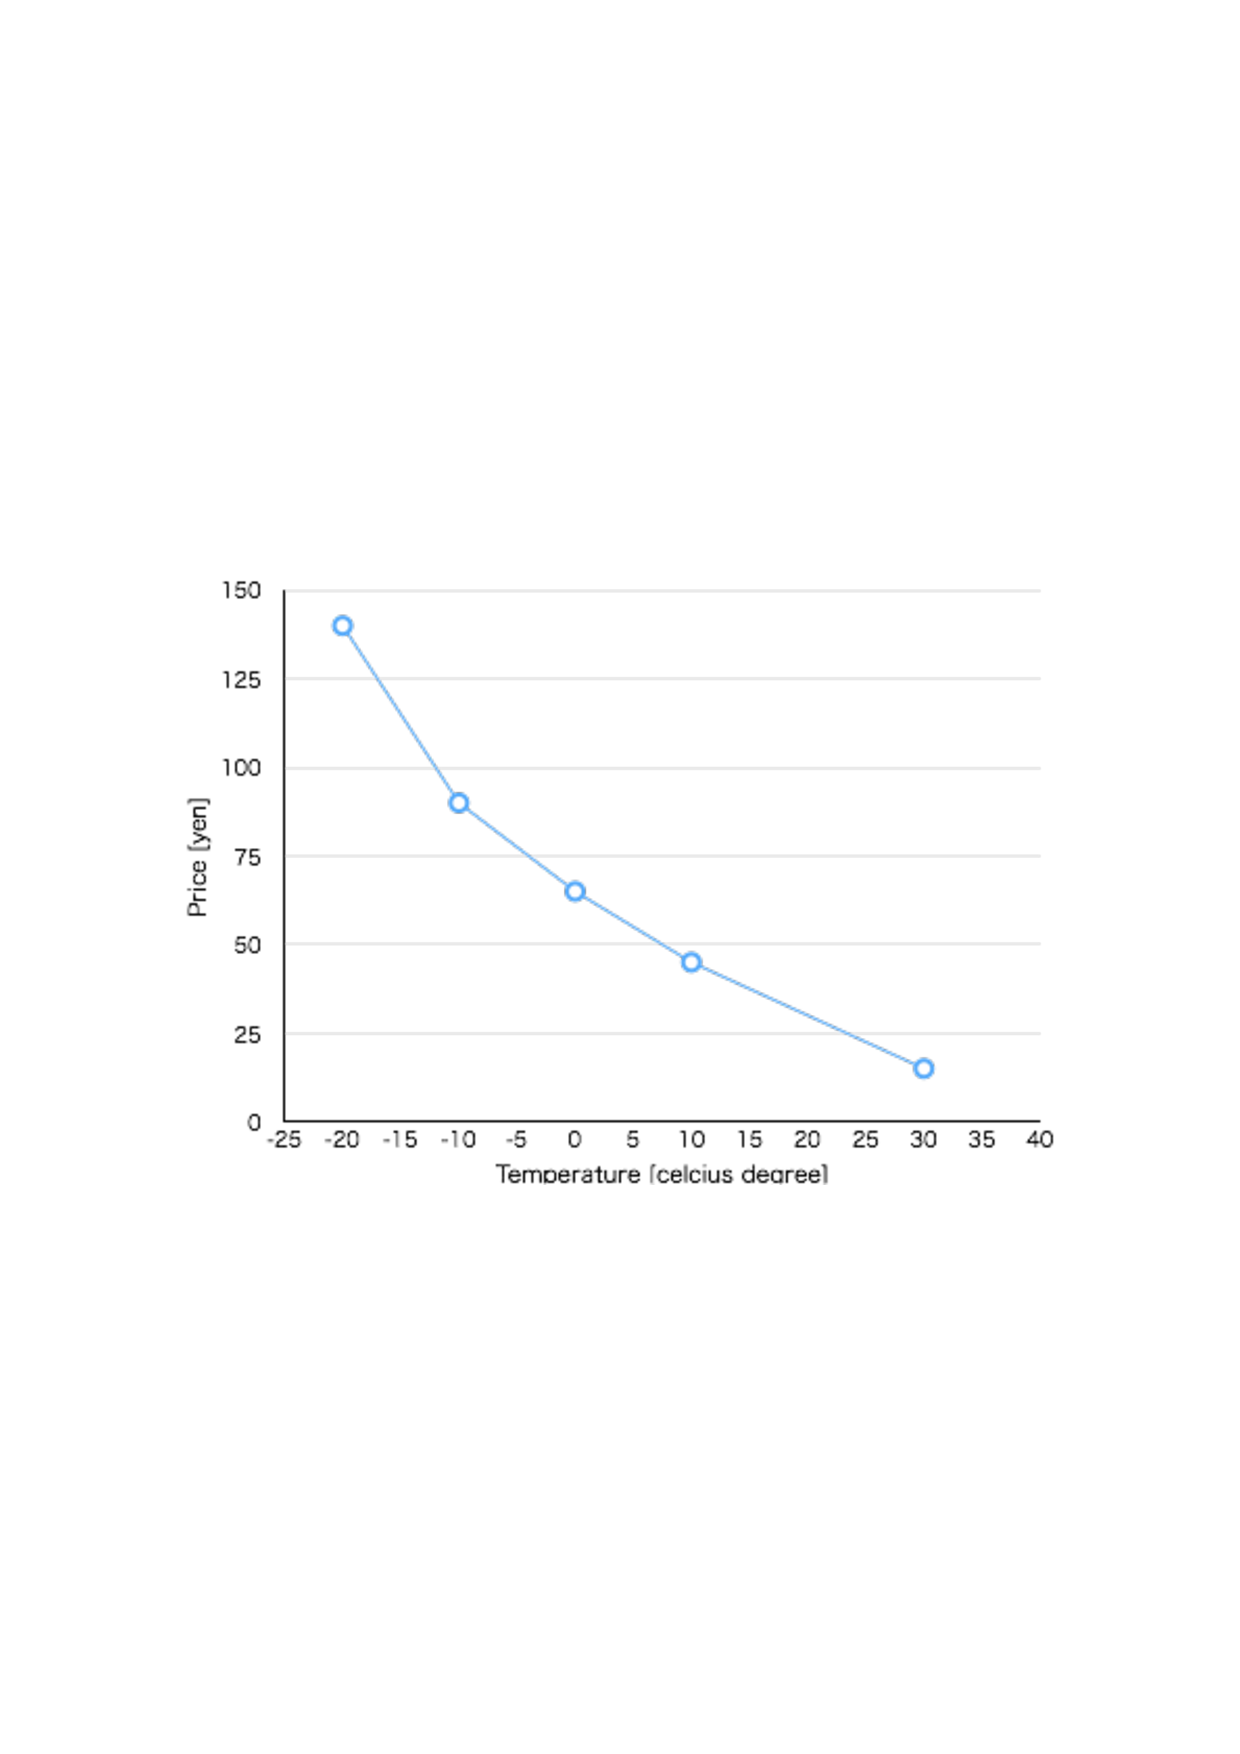
\includegraphics[width=10cm]{images/coolant.pdf}
    \caption{Price of Coolant}
  \end{figure}

  In \verb/calc_cost()/ function, calculate each cost and sum up these.

  \begin{screen}
  \begin{verbatim}
def calc_cost()
  calc electricity_cost by power consumption
  show electricity_cost

  calc toluene_weight
  calc steam_weight by heat balance
  calc steam_cost
  show steam_cost

  calc reactor_price by reactor size
  calc reactor_cost
  show reactor_cost

  calc coolant_weight by total heat of reaction
  calc coolant_cost
  show coolant_cost

  calc total_cost
  show total_cost
end\end{verbatim}
  \end{screen}

  \section{Result}

  \subsection*{(1)$N=1, \gamma_0=0.05, T_2 = 258$}
  Use listing \ref{code:normal},
  \begin{screen}
    \begin{verbatim}
$ ruby reactor.rb
input n[-], gamma_0[wt%], T2[K]
1
0.05
258
elec: 0.106 [yen/s]
steam: 23.455 [yen/s]
reactor: 1.092 [yen/s]
coolant: 2.807 [yen/s]
total: 27.46 [yen/s]\end{verbatim}
  \end{screen}

  \begin{table}[htbp]
    \centering
    \begin{tabular}{cc}\hline
      Electricity Cost & $\SI{0.106}{\yen\per\second}$ \\
      Steam Cost & $\SI{23.455}{\yen\per\second}$ \\
      Reactor Cost & $\SI{1.092}{\yen\per\second}$ \\
      Coolant Cost & $\SI{2.807}{\yen\per\second}$ \\
      Total & $\SI{27.46}{\yen\per\second}$ \\ \hline
    \end{tabular}
    \caption{Result in $(N, \gamma_0, T_2) = (1, 0.05, 258)$}
  \end{table}

  \subsection*{(2)$N=3, \gamma_0=0.04, T_2 = 258$}
  Use listing \ref{code:normal},
  \begin{screen}
    \begin{verbatim}
$ ruby reactor.rb
input n[-], gamma_0[wt%], T2[K]
3
0.04
258
elec: 0.004 [yen/s]
steam: 29.319 [yen/s]
reactor: 2.17 [yen/s]
coolant: 2.706 [yen/s]
total: 34.198 [yen/s]\end{verbatim}
  \end{screen}

  \begin{table}[htbp]
    \centering
    \begin{tabular}{cc}\hline
      Electricity Cost & $\SI{0.004}{\yen\per\second}$ \\
      Steam Cost & $\SI{29.319}{\yen\per\second}$ \\
      Reactor Cost & $\SI{2.17}{\yen\per\second}$ \\
      Coolant Cost & $\SI{2.706}{\yen\per\second}$ \\
      Total & $\SI{34.198}{\yen\per\second}$ \\ \hline
    \end{tabular}
    \caption{Result in $(N, \gamma_0, T_2) = (3, 0.04, 258)$}
  \end{table}

  \subsection*{(3)$N=5, \gamma_0=0.03, T_2 = 300$}
  Use listing \ref{code:normal},
  \begin{screen}
    \begin{verbatim}
$ ruby reactor.rb
input n[-], gamma_0[wt%], T2[K]
5
0.03
300
elec: 0.048 [yen/s]
steam: 39.091 [yen/s]
reactor: 3.321 [yen/s]
coolant: 0.466 [yen/s]
total: 42.927 [yen/s]\end{verbatim}
  \end{screen}

  \begin{table}[htbp]
    \centering
    \begin{tabular}{cc}\hline
      Electricity Cost & $\SI{0.048}{\yen\per\second}$ \\
      Steam Cost & $\SI{39.091}{\yen\per\second}$ \\
      Reactor Cost & $\SI{3.321}{\yen\per\second}$ \\
      Coolant Cost & $\SI{0.466}{\yen\per\second}$ \\
      Total & $\SI{34.198}{\yen\per\second}$ \\ \hline
    \end{tabular}
    \caption{Result in $(N, \gamma_0, T_2) = (5, 0.03, 300)$}
  \end{table}

  \section{Discussion}
  The most major factor deciding cost of product is the cost of steam. So when we optimize cost of product, we should intend to
  minimalize the cost of steam.

  \section{Source Program}
  \lstinputlisting[caption=reactor.rb, label=code:normal]{code/reactor.rb}
\end{document}
